\documentclass{article}
\usepackage{geometry}
\usepackage{graphicx}


\title{Pràctica 4 Llenguatge de Marques}
\author{Francesc Mut Mollà}

\begin{document}
\maketitle
\newpage
\section{Exercici 1}
No hem necessitat de fer cap canvi en el XSD ni en el XML donat que son correctes, es validen.
\vspace{3cm}
\begin{center}
\textit{Comprovant de validació.}
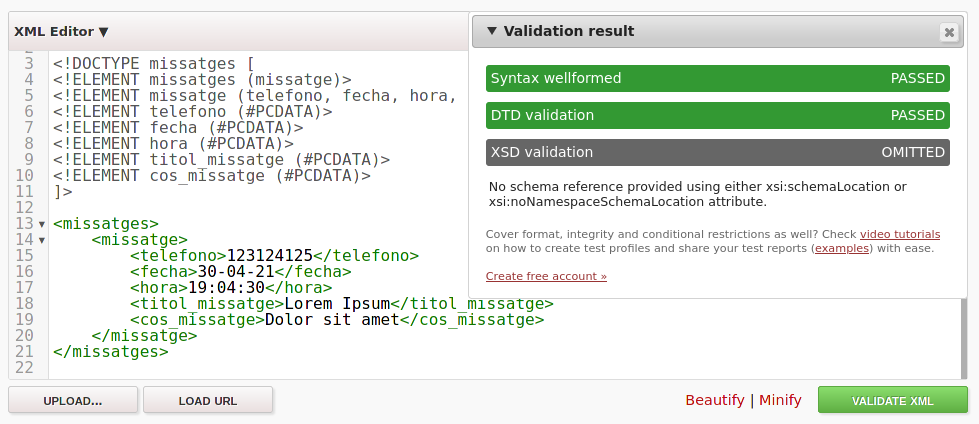
\includegraphics[width=12cm]{validacio1.png}
\end{center}

\newpage


\section{Exercici 2}
He canviat el format de la data per a que s'adeqüi a les restriccions de xs:date, pero segueix donant error encara que té el format AAAA-MM-DD.
\begin{verbatim}
<?xml version="1.0" encoding="UTF-8"?>
<xs:schema xmlns:xs="http://www.w3.org/2001/XMLSchema">
    <xs:element name="persones">
    <xs:complexType>
        <xs:sequence>
            <xs:element name="persona" maxOccurs="unbounded">
              <xs:complexType>
                <xs:sequence>
                  <xs:element name="llinatge" type="xs:string"/>
                  <xs:element name="edat" type="xs:integer"/>
                  <xs:element name="data_naixement" type="xs:date"/>
                 </xs:sequence>
              </xs:complexType>
            </xs:element>
          </xs:sequence>
        </xs:complexType>
    </xs:element>
</xs:schema>
\end{verbatim}
\vspace{0,5cm}
\begin{center}
    \textit{Comprovant de validació.}
    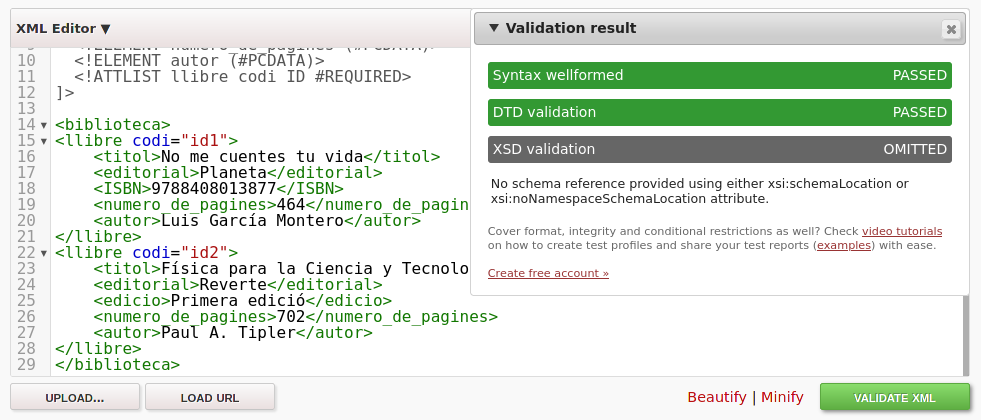
\includegraphics[width=12cm]{validacio2.png}
\end{center}
    
\newpage

\section{Exercici 3}
Es poden aplicar restriccions a l'element fent ús de xs: restrictions dins el simpletype.

\begin{verbatim}
<?xml version="1.0" encoding="UTF-8"?>
<xs:schema xmlns:xs="http://www.w3.org/2001/XMLSchema">
    <xs:element name="edat">
        <xs:simpleType>
            <xs:restriction base="xs:integer">
                <xs:minInclusive value="0" />
                <xs:maxInclusive value="105" />
            </xs:restriction>
        </xs:simpleType>
    </xs:element>
</xs:schema>
\end{verbatim}
\vspace{,5cm}

\section{Exercici 4}

\begin{verbatim}

\end{verbatim}
\vspace{0cm}

\section{Exercici 5}
El tipus sequence ens indica que només es mostraràn en aquest ordre.
\begin{verbatim}
<?xml version="1.0" encoding="UTF-8"?>
<xs:schema xmlns:xs="http://www.w3.org/2001/XMLSchema">
    <xs:complexType name="capell">
        <xs:sequence>
            <xs:element name="color" type="xs:string"></xs:element>
            <xs:element name="model" type="xs:string"></xs:element>
        </xs:sequence>
    </xs:complexType>
</xs:schema>
\end{verbatim}
\vspace{0cm}
\newpage
\section{Exercici 6}
El tipus choice ens permet elegir un tipus o un altre.
\begin{verbatim}
<?xml version="1.0" encoding="UTF-8"?>
<xs:schema xmlns:xs="http://www.w3.org/2001/XMLSchema">
    <xs:complexType name="vehicle">
        <xs:choice>
            <xs:element name="cotxe" type="xs:string"></xs:element>
            <xs:element name="moto" type="xs:string"></xs:element>
            <xs:element name="camió" type="xs:string"></xs:element>
        </xs:choice>
    </xs:complexType>
</xs:schema>
\end{verbatim}
\vspace{0cm}

\section{Exercici 7}
El tipus xs:all ens indica que hi ha de ser tot a l'element.
\begin{verbatim}
<?xml version="1.0" encoding="UTF-8"?>
<xs:schema xmlns:xs="http://www.w3.org/2001/XMLSchema">
    <xs:complexType name="camiseta">
        <xs:all>
            <xs:element name="talla" type="xs:string"></xs:element>
            <xs:element name="color" type="xs:string"></xs:element>
            <xs:element name="preu" type="xs:integer"></xs:element>          
        </xs:all>
    </xs:complexType>
</xs:schema>
\end{verbatim}
\vspace{0cm}
\newpage
\section{Exercici 8}

\begin{verbatim}
<?xml version="1.0" encoding="UTF-8"?>
<xs:schema xmlns:xs="http://www.w3.org/2001/XMLSchema">
  <xs:element name="empleat">
    <xs:complexType>
      <xs:sequence>
        <xs:element name="nom" type="xs:string"></xs:element>
        <xs:element name="direccio" maxOccurs="unbounded">
          <xs:complexType>
            <xs:sequence>
              <xs:element name="carrer" type="xs:string"/>
              <xs:element name="numero" type="xs:integer"/>
              <xs:element name="ciutat" type="xs:string"/>
              <xs:element name="provincia" type="xs:string"></xs:element>
             </xs:sequence>
          </xs:complexType>
        </xs:element>
        <xs:element name="telefono">
            <xs:simpleType>
                <xs:restriction base="xs:integer">
                  <xs:totalDigits value="9"/>
                </xs:restriction>
              </xs:simpleType>
        </xs:element>
      </xs:sequence>
    <xs:attribute name="codi" type="xs:string" use="required"/>
    </xs:complexType>
  </xs:element>
</xs:schema>
\end{verbatim}
\vspace{0cm}
\begin{center}
    \textit{Comprovant de validació.}
    \includegraphics[width=12cm]{validacio8.png}
\end{center}
\section{Exercici 9}

\begin{verbatim}
<?xml version="1.0" encoding="UTF-8"?>
<xs:schema xmlns:xs="http://www.w3.org/2001/XMLSchema">
  <xs:element name="pelicula">
    <xs:complexType>
      <xs:sequence>
        <xs:element name="director" type="xs:string"></xs:element>
        <xs:element name="repartiment" maxOccurs="unbounded">
          <xs:complexType>
            <xs:sequence>
              <xs:element name="interpret" type="xs:string" maxOccurs="unbounded"/>
             </xs:sequence>
          </xs:complexType>
        </xs:element>
      </xs:sequence>
    <xs:attribute name="titol" type="xs:string" use="required"/>
    <xs:attribute name="minuts" type="xs:integer" use="required"/>
    </xs:complexType>
  </xs:element>
</xs:schema>
\end{verbatim}
\vspace{0cm}
\begin{center}
    \textit{Comprovant de validació.}
    \includegraphics[width=12cm]{validacio9.png}
\end{center}
\newpage
\section{Exercici 10}
Tinc un error de validació a la línia 26 que no he pogut solucionar, no em deixa aplicar la restricció. A més, encara tenc l'error de la data de l'exercici anterior.
\begin{verbatim}
<?xml version="1.0" encoding="UTF-8"?>
<xs:schema xmlns:xs="http://www.w3.org/2001/XMLSchema">
    <xs:element name="institut">
        <xs:complexType>
            <xs:sequence>
                <xs:element name="alumne" maxOccurs="unbounded">
                    <xs:complexType>
                        <xs:sequence>
                            <xs:element name="dades" maxOccurs="1">
                                <xs:complexType>
                                    <xs:sequence>
                                        <xs:element name="nom" type="xs:string" />
                                        <xs:element name="llinatge" type="xs:string" />
                                        <xs:element name="dni" maxOccurs="unbounded">
                                            <xs:simpleType>
                                                <xs:restriction base="xs:integer">
                                                    <xs:totalDigits value="9" />
                                                </xs:restriction>
                                            </xs:simpleType>
                                        </xs:element>
                                    </xs:sequence>
                                </xs:complexType>
                            </xs:element>
                            <xs:element name="comentaris" maxOccurs="1" minOccurs="0">
                                <xs:simpleType>
                                    <xs:restriction>
                                        <xs:minLength value="5"></xs:minLength>
                                        <xs:maxLength value="50"></xs:maxLength>
                                    </xs:restriction>
                                </xs:simpleType>
                            </xs:element>
                        </xs:sequence>
                    </xs:complexType>
                </xs:element>
            </xs:sequence>
            <xs:attribute name="titol" type="xs:string" use="required" />
            <xs:attribute name="minuts" type="xs:integer" use="required" />
        </xs:complexType>
    </xs:element>
</xs:schema>
\end{verbatim}
\vspace{1cm}
\begin{center}
    \textit{Comprovant de validació.}
    \includegraphics[width=12cm]{validacio10.png}
\end{center}
\end{document}